\documentclass[aspectratio=169,11pt]{beamer}

% Compile with XeLaTeX
\usepackage{fontspec}
\setsansfont{DejaVu Sans}
\setmonofont{DejaVu Sans Mono}
\usepackage{polyglossia}
\setdefaultlanguage{vietnamese}
\usepackage{booktabs}
\usepackage{array}
\usepackage{tabularx}
\usepackage{xcolor}
\usepackage{ragged2e}
\usepackage{tikz}
\usetikzlibrary{positioning,arrows.meta,shapes.geometric}

% Graphics
\usepackage{graphicx}
\graphicspath{{images/}}

\usetheme{Madrid}
\usecolortheme{seahorse}
\setbeamertemplate{navigation symbols}{}
\setbeamertemplate{footline}[frame number]
\setbeamertemplate{itemize items}[circle]
\setbeamertemplate{enumerate items}[default]

\definecolor{accent}{RGB}{0,90,150}
\definecolor{softblue}{RGB}{220,235,250}
\definecolor{softgreen}{RGB}{224,245,232}
\definecolor{softorange}{RGB}{255,238,215}
\definecolor{softred}{RGB}{252,225,225}
\definecolor{darkblue}{RGB}{0,72,128}

\newcommand{\keyword}[1]{\textcolor{accent}{\textbf{#1}}}
\newcommand{\tightlist}{\setlength{\itemsep}{2pt}\setlength{\parskip}{0pt}}
\newcommand{\qoption}[2]{\item[#1.] #2}

\title[Các loại kiến trúc DBMS]{Các loại kiến trúc DBMS}
\subtitle{1-Tier, 2-Tier và 3-Tier Architecture}
\author{Tài liệu bài giảng}
\institute{Môn học: Cơ sở dữ liệu}
\date{Cập nhật: 24/04/2026}

\begin{document}

%------------------------------------------------
\begin{frame}
  \titlepage
\end{frame}

%------------------------------------------------
\begin{frame}{Mục tiêu bài giảng}
\small
Sau khi hoàn thành bài học này, người học có thể:
\begin{enumerate}
\tightlist
  \item Trình bày khái niệm \keyword{kiến trúc DBMS}.
  \item Phân biệt các mô hình kiến trúc \keyword{1 tầng}, \keyword{2 tầng} và \keyword{3 tầng}.
  \item Giải thích vai trò của từng tầng trong hệ thống cơ sở dữ liệu.
  \item Phân tích ưu điểm và nhược điểm của từng loại kiến trúc DBMS.
  \item Lựa chọn kiến trúc DBMS phù hợp cho một số tình huống ứng dụng thực tế.
\end{enumerate}
\end{frame}

%------------------------------------------------
\begin{frame}{Kiến trúc DBMS là gì?}
\small
\begin{block}{Định nghĩa}
\keyword{Kiến trúc DBMS} mô tả cách người dùng và ứng dụng tương tác với cơ sở dữ liệu để \textbf{đọc}, \textbf{ghi}, \textbf{cập nhật} hoặc \textbf{truy vấn} thông tin.
\end{block}

Một kiến trúc DBMS được thiết kế tốt giúp hệ thống:
\begin{itemize}
\tightlist
  \item Đảm bảo tính nhất quán của dữ liệu.
  \item Cải thiện hiệu năng xử lý.
  \item Tăng cường bảo mật dữ liệu.
  \item Hỗ trợ nhiều người dùng và nhiều ứng dụng cùng truy cập dữ liệu.
  \item Dễ bảo trì và mở rộng hệ thống.
\end{itemize}
\end{frame}

%------------------------------------------------
\begin{frame}{Schema trong kiến trúc DBMS}
\small
\begin{block}{Schema}
\keyword{Schema} hay \keyword{lược đồ cơ sở dữ liệu} là bản thiết kế mô tả cách dữ liệu được tổ chức trong hệ thống.
\end{block}

Schema thường mô tả:
\begin{itemize}
\tightlist
  \item Các bảng dữ liệu.
  \item Các trường dữ liệu.
  \item Kiểu dữ liệu.
  \item Khóa chính và khóa ngoại.
  \item Quan hệ giữa các bảng.
\end{itemize}

\begin{exampleblock}{Ghi nhớ}
Kiến trúc DBMS nói về cách các thành phần hệ thống tương tác; schema nói về cách dữ liệu được tổ chức bên trong cơ sở dữ liệu.
\end{exampleblock}
\end{frame}

%------------------------------------------------
\section{Kiến trúc 1 tầng}

\begin{frame}{Kiến trúc 1 tầng: Khái niệm}
\small
Trong kiến trúc \keyword{1 tầng} (\textit{1-Tier Architecture}), người dùng làm việc trực tiếp với cơ sở dữ liệu trên cùng một hệ thống.

\vspace{0.2cm}
Điều này có nghĩa là các thành phần sau nằm trong cùng một ứng dụng hoặc cùng một máy tính:
\begin{itemize}
\tightlist
  \item Giao diện người dùng.
  \item Logic xử lý.
  \item Dữ liệu.
\end{itemize}

Người dùng có thể mở ứng dụng, nhập dữ liệu, xử lý dữ liệu và lưu trữ dữ liệu trực tiếp mà không cần máy chủ riêng hoặc kết nối mạng.
\end{frame}

%------------------------------------------------
\begin{frame}{Sơ đồ kiến trúc 1 tầng}
\centering
\vfill
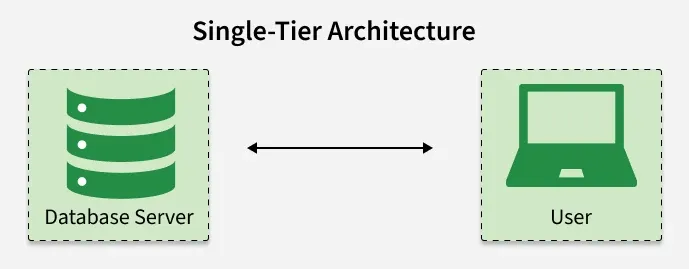
\includegraphics[width=0.78\textwidth,height=0.68\textheight,keepaspectratio]{image-1.png}
\vfill
\vspace{0.25cm}
\small \textit{Giao diện, logic xử lý và dữ liệu nằm trong cùng một máy tính / một ứng dụng.}
\end{frame}

%------------------------------------------------
\begin{frame}{Ví dụ về kiến trúc 1 tầng}
\small
\begin{block}{Ví dụ phổ biến}
\keyword{Microsoft Access} là một ví dụ thường gặp của kiến trúc 1 tầng.
\end{block}

Trong MS Access:
\begin{itemize}
\tightlist
  \item Người dùng nhập dữ liệu trực tiếp.
  \item Ứng dụng xử lý các thao tác tính toán hoặc truy vấn.
  \item Dữ liệu được lưu trực tiếp trên máy tính cá nhân.
  \item Không cần máy chủ cơ sở dữ liệu riêng.
\end{itemize}

\begin{exampleblock}{Phù hợp với}
Ứng dụng cá nhân, ứng dụng độc lập, bài thực hành nhỏ hoặc hệ thống quy mô nhỏ.
\end{exampleblock}
\end{frame}

%------------------------------------------------
\begin{frame}{Kiến trúc 1 tầng: Ưu điểm}
\small
\begin{itemize}
\tightlist
  \item \keyword{Đơn giản}: chỉ cần một máy tính để cài đặt, vận hành và bảo trì.
  \item \keyword{Chi phí thấp}: không cần máy chủ, hạ tầng mạng hoặc phần cứng phức tạp.
  \item \keyword{Dễ triển khai}: phù hợp với dự án nhỏ, bài thực hành cá nhân hoặc ứng dụng nội bộ đơn giản.
  \item \keyword{Không phụ thuộc vào mạng}: người dùng có thể làm việc trực tiếp trên máy cá nhân.
\end{itemize}
\end{frame}

%------------------------------------------------
\begin{frame}{Kiến trúc 1 tầng: Nhược điểm}
\small
\begin{itemize}
\tightlist
  \item \keyword{Chỉ phù hợp với một người dùng}: không tốt cho làm việc nhóm hoặc môi trường nhiều người dùng.
  \item \keyword{Bảo mật kém}: ứng dụng và dữ liệu nằm trên cùng một máy.
  \item \keyword{Không có kiểm soát tập trung}: dữ liệu lưu cục bộ, khó quản lý và sao lưu tập trung.
  \item \keyword{Khó chia sẻ dữ liệu}: dữ liệu nằm trên một máy tính nên khó chia sẻ giữa nhiều thiết bị.
\end{itemize}
\end{frame}

%------------------------------------------------
\begin{frame}{Quiz: Kiến trúc 1 tầng}
\small
\textbf{Câu 1.} Trong kiến trúc 1 tầng, các thành phần nào thường nằm trên cùng một máy?
\begin{enumerate}
\tightlist
  \qoption{A}{Chỉ cơ sở dữ liệu}
  \qoption{B}{Chỉ giao diện người dùng}
  \qoption{C}{Giao diện, logic xử lý và dữ liệu}
  \qoption{D}{Chỉ máy chủ ứng dụng}
\end{enumerate}

\textbf{Câu 2.} Ví dụ nào sau đây phù hợp nhất với kiến trúc 1 tầng?
\begin{enumerate}
\tightlist
  \qoption{A}{Hệ thống thương mại điện tử lớn}
  \qoption{B}{Ứng dụng MS Access chạy trên máy cá nhân}
  \qoption{C}{Hệ thống ngân hàng trực tuyến}
  \qoption{D}{Hệ thống mạng xã hội}
\end{enumerate}
\end{frame}

%------------------------------------------------
\begin{frame}{Quiz: Kiến trúc 1 tầng (tiếp)}
\small
\textbf{Câu 3.} Nhược điểm lớn của kiến trúc 1 tầng là gì?
\begin{enumerate}
\tightlist
  \qoption{A}{Quá phức tạp}
  \qoption{B}{Không thể lưu dữ liệu}
  \qoption{C}{Khó hỗ trợ nhiều người dùng}
  \qoption{D}{Không thể chạy trên máy cá nhân}
\end{enumerate}
\end{frame}

%------------------------------------------------
\section{Kiến trúc 2 tầng}

\begin{frame}{Kiến trúc 2 tầng: Khái niệm}
\small
Kiến trúc \keyword{2 tầng} (\textit{2-Tier Architecture}) tương tự mô hình \keyword{client-server} cơ bản.

\vspace{0.2cm}
Trong mô hình này:
\begin{itemize}
\tightlist
  \item \keyword{Client}: chạy giao diện người dùng và chương trình ứng dụng.
  \item \keyword{Database Server}: lưu trữ và xử lý dữ liệu.
\end{itemize}

Ứng dụng phía client giao tiếp trực tiếp với cơ sở dữ liệu ở phía server. Các API như \keyword{ODBC} và \keyword{JDBC} thường được dùng để hỗ trợ kết nối.
\end{frame}

%------------------------------------------------
\begin{frame}{Sơ đồ kiến trúc 2 tầng}
\centering
\vfill
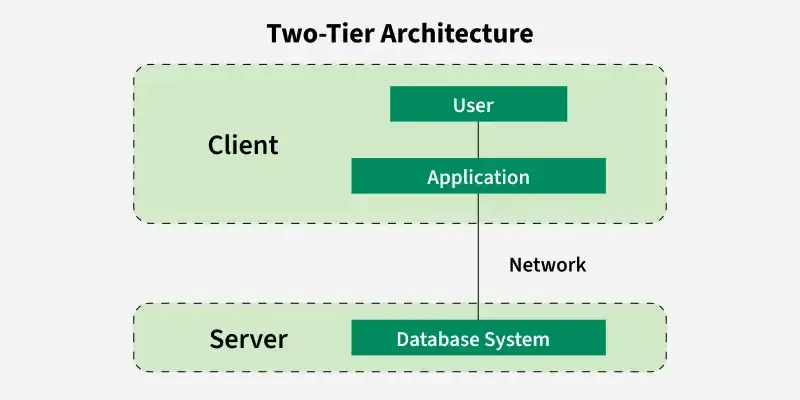
\includegraphics[width=0.78\textwidth,height=0.68\textheight,keepaspectratio]{image-2.png}
\vfill
\vspace{0.5cm}
\small Client kết nối trực tiếp đến database server để gửi truy vấn và nhận kết quả.
\end{frame}


%------------------------------------------------
\begin{frame}{Ví dụ: Hệ thống quản lý thư viện}
\small
\begin{columns}[T]
\column{0.48\textwidth}
\begin{block}{Tầng client}
Ứng dụng desktop để nhân viên thư viện hoặc người dùng:
\begin{itemize}
\tightlist
  \item Tìm kiếm sách.
  \item Mượn sách.
  \item Trả sách.
  \item Kiểm tra hạn trả.
\end{itemize}
\end{block}

\column{0.48\textwidth}
\begin{block}{Tầng cơ sở dữ liệu}
Database server lưu trữ:
\begin{itemize}
\tightlist
  \item Thông tin sách.
  \item Thông tin người dùng.
  \item Lịch sử mượn trả.
  \item Nhật ký giao dịch.
\end{itemize}
\end{block}
\end{columns}
\end{frame}

%------------------------------------------------
\begin{frame}{Kiến trúc 2 tầng: Ưu điểm}
\small
\begin{itemize}
\tightlist
  \item \keyword{Truy cập dữ liệu nhanh}: client có thể gửi truy vấn trực tiếp đến server.
  \item \keyword{Chi phí thấp hơn 3 tầng}: không cần tầng ứng dụng trung gian.
  \item \keyword{Dễ triển khai}: mô hình chỉ gồm client và database server.
  \item \keyword{Đơn giản}: phù hợp với hệ thống nhỏ hoặc vừa trong mạng nội bộ.
\end{itemize}
\end{frame}

%------------------------------------------------
\begin{frame}{Kiến trúc 2 tầng: Nhược điểm}
\small
\begin{itemize}
\tightlist
  \item \keyword{Khả năng mở rộng hạn chế}: server có thể quá tải khi số lượng client tăng.
  \item \keyword{Vấn đề bảo mật}: client kết nối trực tiếp đến cơ sở dữ liệu.
  \item \keyword{Liên kết chặt}: nếu database thay đổi, client thường cũng phải cập nhật.
  \item \keyword{Khó bảo trì}: quản lý cập nhật, sửa lỗi và thêm chức năng khó hơn khi số lượng client tăng.
\end{itemize}
\end{frame}

%------------------------------------------------
\begin{frame}{Quiz: Kiến trúc 2 tầng}
\small
\textbf{Câu 1.} Kiến trúc 2 tầng gồm hai tầng chính nào?
\begin{enumerate}
\tightlist
  \qoption{A}{Client và database server}
  \qoption{B}{Client và trình duyệt web}
  \qoption{C}{Database và hệ điều hành}
  \qoption{D}{Ứng dụng và tệp văn bản}
\end{enumerate}

\textbf{Câu 2.} Trong kiến trúc 2 tầng, client thường giao tiếp với cơ sở dữ liệu thông qua công nghệ nào?
\begin{enumerate}
\tightlist
  \qoption{A}{HTML và CSS}
  \qoption{B}{ODBC hoặc JDBC}
  \qoption{C}{Bluetooth}
  \qoption{D}{FTP}
\end{enumerate}
\end{frame}

%------------------------------------------------
\begin{frame}{Quiz: Kiến trúc 2 tầng (tiếp)}
\small
\textbf{Câu 3.} Nhược điểm bảo mật của kiến trúc 2 tầng là gì?
\begin{enumerate}
\tightlist
  \qoption{A}{Không lưu được dữ liệu}
  \qoption{B}{Client kết nối trực tiếp với cơ sở dữ liệu}
  \qoption{C}{Không có giao diện người dùng}
  \qoption{D}{Không thể xử lý truy vấn}
\end{enumerate}
\end{frame}

%------------------------------------------------
\section{Kiến trúc 3 tầng}

\begin{frame}{Kiến trúc 3 tầng: Khái niệm}
\small
Trong kiến trúc \keyword{3 tầng} (\textit{3-Tier Architecture}), có thêm một tầng trung gian giữa client và database server.

\vspace{0.2cm}
Ba tầng chính gồm:
\begin{enumerate}
\tightlist
  \item \keyword{Presentation Layer}: tầng trình bày.
  \item \keyword{Application / Business Logic Layer}: tầng ứng dụng hoặc xử lý nghiệp vụ.
  \item \keyword{Database Layer}: tầng cơ sở dữ liệu.
\end{enumerate}

Client không giao tiếp trực tiếp với database. Thay vào đó, client gửi yêu cầu đến application server.
\end{frame}

%------------------------------------------------
\begin{frame}{Sơ đồ kiến trúc 3 tầng}
\centering
\vfill
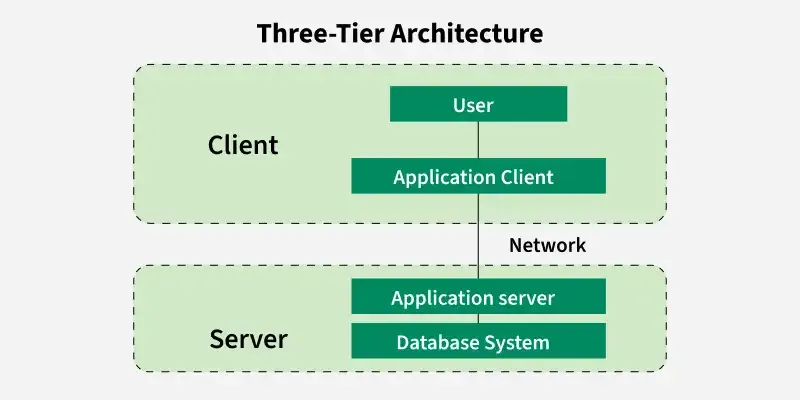
\includegraphics[width=0.78\textwidth,height=0.68\textheight,keepaspectratio]{image-3.png}
\vfill
\vspace{0.5cm}
\small Tầng ứng dụng đóng vai trò trung gian, kiểm soát logic nghiệp vụ và truy cập dữ liệu.
\end{frame}

%------------------------------------------------
\begin{frame}{Luồng xử lý trong kiến trúc 3 tầng}
\small
\begin{enumerate}
\tightlist
  \item Client gửi yêu cầu đến application server.
  \item Application server xử lý logic nghiệp vụ.
  \item Application server gửi truy vấn đến database server khi cần.
  \item Database server trả dữ liệu về application server.
  \item Application server xử lý kết quả và gửi phản hồi về client.
\end{enumerate}

\begin{block}{Ứng dụng phổ biến}
Kiến trúc 3 tầng thường dùng trong ứng dụng web lớn, hệ thống doanh nghiệp, thương mại điện tử, ngân hàng trực tuyến và hệ thống nhiều người dùng truy cập đồng thời.
\end{block}
\end{frame}

%------------------------------------------------
\begin{frame}{Ví dụ: Cửa hàng thương mại điện tử}
\small
\begin{columns}[T]
\column{0.33\textwidth}
\begin{block}{Người dùng}
\begin{itemize}
\tightlist
  \item Truy cập website.
  \item Tìm kiếm sản phẩm.
  \item Thêm vào giỏ hàng.
\end{itemize}
\end{block}

\column{0.33\textwidth}
\begin{block}{Tầng xử lý}
\begin{itemize}
\tightlist
  \item Kiểm tra tồn kho.
  \item Tính tổng giá.
  \item Áp dụng giảm giá.
  \item Xác thực tài khoản.
\end{itemize}
\end{block}

\column{0.33\textwidth}
\begin{block}{Tầng dữ liệu}
\begin{itemize}
\tightlist
  \item Sản phẩm.
  \item Khách hàng.
  \item Giỏ hàng.
  \item Đơn hàng.
\end{itemize}
\end{block}
\end{columns}
\end{frame}

%------------------------------------------------
\begin{frame}{Kiến trúc 3 tầng: Ưu điểm}
\small
\begin{itemize}
\tightlist
  \item \keyword{Khả năng mở rộng tốt}: tầng ứng dụng có thể triển khai phân tán trên nhiều server.
  \item \keyword{Tăng tính toàn vẹn dữ liệu}: tầng trung gian kiểm soát dữ liệu trước khi gửi đến database.
  \item \keyword{Bảo mật tốt hơn}: client không truy cập trực tiếp vào cơ sở dữ liệu.
  \item \keyword{Dễ bảo trì}: logic nghiệp vụ nằm ở tầng ứng dụng.
  \item \keyword{Phù hợp với ứng dụng lớn}: hỗ trợ nhiều người dùng, nhiều chức năng và yêu cầu bảo mật cao.
\end{itemize}
\end{frame}

%------------------------------------------------
\begin{frame}{Kiến trúc 3 tầng: Nhược điểm}
\small
\begin{itemize}
\tightlist
  \item \keyword{Phức tạp hơn}: có thêm tầng trung gian so với 2 tầng.
  \item \keyword{Khó thiết kế giao tiếp}: dữ liệu phải đi qua nhiều tầng.
  \item \keyword{Thời gian phản hồi có thể chậm hơn}: yêu cầu đi qua application server.
  \item \keyword{Chi phí cao hơn}: cần phần cứng, phần mềm và nhân lực có chuyên môn.
\end{itemize}
\end{frame}

%------------------------------------------------
\begin{frame}{Quiz: Kiến trúc 3 tầng}
\small
\textbf{Câu 1.} Ba tầng chính trong kiến trúc 3 tầng là gì?
\begin{enumerate}
\tightlist
  \qoption{A}{File, folder, disk}
  \qoption{B}{Client, application server, database server}
  \qoption{C}{RAM, CPU, hard disk}
  \qoption{D}{User, password, table}
\end{enumerate}

\textbf{Câu 2.} Trong kiến trúc 3 tầng, client có kết nối trực tiếp với database không?
\begin{enumerate}
\tightlist
  \qoption{A}{Có}
  \qoption{B}{Không}
  \qoption{C}{Chỉ khi database nhỏ}
  \qoption{D}{Chỉ khi dùng MS Access}
\end{enumerate}
\end{frame}

%------------------------------------------------
\begin{frame}{Quiz: Kiến trúc 3 tầng (tiếp)}
\small
\textbf{Câu 3.} Lợi ích bảo mật chính của kiến trúc 3 tầng là gì?
\begin{enumerate}
\tightlist
  \qoption{A}{Không cần mật khẩu}
  \qoption{B}{Client không truy cập trực tiếp vào cơ sở dữ liệu}
  \qoption{C}{Không cần máy chủ}
  \qoption{D}{Dữ liệu được lưu trên giấy}
\end{enumerate}
\end{frame}

%------------------------------------------------
\section{So sánh và lựa chọn}

\begin{frame}{So sánh nhanh ba loại kiến trúc}
\scriptsize
\begin{tabularx}{\textwidth}{p{0.20\textwidth} X X X}
\toprule
\textbf{Tiêu chí} & \textbf{1 tầng} & \textbf{2 tầng} & \textbf{3 tầng} \\
\midrule
Số tầng & 1 & 2 & 3 \\
Thành phần & Ứng dụng và dữ liệu cùng một máy & Client và database server & Client, application server, database server \\
Truy cập dữ liệu & Trực tiếp trên máy cục bộ & Client trực tiếp đến database server & Thông qua application server \\
Ví dụ & MS Access cá nhân & Quản lý thư viện nhỏ & Website thương mại điện tử \\
Khả năng mở rộng & Thấp & Trung bình & Cao \\
Bảo mật & Thấp & Trung bình & Tốt hơn \\
\bottomrule
\end{tabularx}
\end{frame}

%------------------------------------------------
\begin{frame}{Khi nào nên chọn từng kiến trúc?}
\small
\begin{columns}[T]
\column{0.32\textwidth}
\begin{block}{1 tầng}
\begin{itemize}
\tightlist
  \item Ứng dụng cá nhân.
  \item Dữ liệu nhỏ.
  \item Một người dùng.
  \item Chi phí thấp.
\end{itemize}
\end{block}

\column{0.32\textwidth}
\begin{block}{2 tầng}
\begin{itemize}
\tightlist
  \item Tổ chức nhỏ/vừa.
  \item Mạng nội bộ.
  \item Ứng dụng desktop.
  \item Client kết nối DB.
\end{itemize}
\end{block}

\column{0.32\textwidth}
\begin{block}{3 tầng}
\begin{itemize}
\tightlist
  \item Web app lớn.
  \item Nhiều người dùng.
  \item Bảo mật cao.
  \item Dễ mở rộng.
\end{itemize}
\end{block}
\end{columns}
\end{frame}

%------------------------------------------------
\begin{frame}{Câu hỏi ôn tập: Trắc nghiệm 1-5}
\small
\textbf{Câu 1.} Kiến trúc DBMS mô tả điều gì?
\begin{enumerate}\tightlist
  \qoption{A}{Cách thiết kế giao diện đồ họa}
  \qoption{B}{Cách người dùng và ứng dụng tương tác với cơ sở dữ liệu}
  \qoption{C}{Cách lắp ráp phần cứng máy tính}
  \qoption{D}{Cách định dạng văn bản}
\end{enumerate}

\textbf{Câu 2.} Kiến trúc nào phù hợp nhất với ứng dụng cá nhân, không cần mạng?
\begin{enumerate}\tightlist
  \qoption{A}{1 tầng} \qoption{B}{2 tầng} \qoption{C}{3 tầng} \qoption{D}{Nhiều tầng}
\end{enumerate}

\textbf{Câu 3.} Trong kiến trúc 2 tầng, tầng client thường chứa thành phần nào?
\begin{enumerate}\tightlist
  \qoption{A}{Giao diện người dùng và chương trình ứng dụng}
  \qoption{B}{Chỉ dữ liệu thô}
  \qoption{C}{Chỉ ổ cứng}
  \qoption{D}{Chỉ hệ điều hành}
\end{enumerate}
\end{frame}

%------------------------------------------------
\begin{frame}{Câu hỏi ôn tập: Trắc nghiệm 4-6}
\small
\textbf{Câu 4.} Trong kiến trúc 3 tầng, tầng nào thường xử lý logic nghiệp vụ?
\begin{enumerate}\tightlist
  \qoption{A}{Tầng trình bày}
  \qoption{B}{Tầng ứng dụng}
  \qoption{C}{Tầng cơ sở dữ liệu}
  \qoption{D}{Tầng lưu trữ vật lý}
\end{enumerate}

\textbf{Câu 5.} Nhược điểm chính của kiến trúc 1 tầng là gì?
\begin{enumerate}\tightlist
  \qoption{A}{Không có khả năng lưu trữ dữ liệu}
  \qoption{B}{Khó hỗ trợ nhiều người dùng và bảo mật thấp}
  \qoption{C}{Luôn cần nhiều máy chủ}
  \qoption{D}{Không thể dùng cho ứng dụng nhỏ}
\end{enumerate}

\textbf{Câu 6.} Lý do kiến trúc 3 tầng có khả năng bảo mật tốt hơn là gì?
\begin{enumerate}\tightlist
  \qoption{A}{Vì không cần database}
  \qoption{B}{Vì client không truy cập trực tiếp vào database}
  \qoption{C}{Vì dữ liệu không được lưu trữ}
  \qoption{D}{Vì không có tầng ứng dụng}
\end{enumerate}
\end{frame}

%------------------------------------------------
\begin{frame}{Câu hỏi ôn tập: Trắc nghiệm 7-8}
\small
\textbf{Câu 7.} Ví dụ nào phù hợp nhất với kiến trúc 3 tầng?
\begin{enumerate}\tightlist
  \qoption{A}{File Excel lưu trên máy cá nhân}
  \qoption{B}{MS Access dùng cho một người}
  \qoption{C}{Website thương mại điện tử}
  \qoption{D}{Tệp văn bản lưu trong USB}
\end{enumerate}

\textbf{Câu 8.} Trong kiến trúc 2 tầng, khi số lượng người dùng tăng mạnh, vấn đề nào có thể xảy ra?
\begin{enumerate}\tightlist
  \qoption{A}{Server bị quá tải do nhiều kết nối trực tiếp}
  \qoption{B}{Client không còn giao diện}
  \qoption{C}{Database tự động biến mất}
  \qoption{D}{Không thể tạo bảng}
\end{enumerate}
\end{frame}

%------------------------------------------------
%------------------------------------------------
\begin{frame}{Câu hỏi ôn tập: Trắc nghiệm 9-10}
\small
\textbf{Câu 9.} ODBC và JDBC thường được dùng trong kiến trúc nào?
\begin{enumerate}\tightlist
  \qoption{A}{1 tầng}
  \qoption{B}{2 tầng}
  \qoption{C}{3 tầng}
  \qoption{D}{Không liên quan đến DBMS}
\end{enumerate}

\textbf{Câu 10.} Kiến trúc nào thường phù hợp nhất cho hệ thống doanh nghiệp lớn?
\begin{enumerate}\tightlist
  \qoption{A}{1 tầng}
  \qoption{B}{2 tầng}
  \qoption{C}{3 tầng}
  \qoption{D}{File-based system}
\end{enumerate}
\end{frame}

%------------------------------------------------
\begin{frame}{Câu hỏi ôn tập: Tự luận ngắn}
\small
\begin{enumerate}\tightlist
  \item Vì sao kiến trúc 1 tầng không phù hợp với hệ thống có nhiều người dùng?
  \item Phân biệt kiến trúc 2 tầng và 3 tầng về cách client truy cập cơ sở dữ liệu.
  \item Vì sao kiến trúc 3 tầng thường được dùng cho ứng dụng web lớn?
  \item Nêu một ví dụ thực tế cho từng loại kiến trúc DBMS.
\end{enumerate}
\end{frame}

%------------------------------------------------
%------------------------------------------------
\begin{frame}{Bài tập vận dụng 1}
\small
\begin{block}{Tình huống}
Một cửa hàng nhỏ muốn quản lý danh sách sản phẩm và doanh thu bán hàng trên một máy tính cá nhân. Cửa hàng chỉ có một người dùng hệ thống.
\end{block}

\begin{exampleblock}{Yêu cầu}
Hãy đề xuất kiến trúc DBMS phù hợp và giải thích lý do.
\end{exampleblock}
\end{frame}

%------------------------------------------------
\begin{frame}{Bài tập vận dụng 2}
\small
\begin{block}{Tình huống}
Một thư viện trường học muốn xây dựng phần mềm desktop để nhiều nhân viên có thể tra cứu sách và cập nhật thông tin mượn trả. Dữ liệu được lưu trên một máy chủ trong mạng nội bộ.
\end{block}

\begin{exampleblock}{Yêu cầu}
Hãy đề xuất kiến trúc DBMS phù hợp và giải thích lý do.
\end{exampleblock}
\end{frame}

%------------------------------------------------
\begin{frame}{Bài tập vận dụng 3}
\small
\begin{block}{Tình huống}
Một công ty muốn xây dựng website thương mại điện tử phục vụ hàng nghìn người dùng truy cập cùng lúc. Hệ thống cần bảo mật, xử lý đơn hàng, kiểm tra tồn kho và lưu lịch sử mua hàng.
\end{block}

\begin{exampleblock}{Yêu cầu}
Hãy đề xuất kiến trúc DBMS phù hợp và giải thích lý do.
\end{exampleblock}
\end{frame}

%------------------------------------------------
\begin{frame}{Tóm tắt bài học}
\small
\begin{itemize}
\tightlist
  \item Kiến trúc DBMS mô tả cách người dùng, ứng dụng và cơ sở dữ liệu tương tác với nhau.
  \item Kiến trúc 1 tầng đơn giản, chi phí thấp nhưng khó mở rộng và bảo mật thấp.
  \item Kiến trúc 2 tầng gồm client và database server, phù hợp với hệ thống nhỏ hoặc vừa.
  \item Kiến trúc 3 tầng bổ sung application server, giúp tăng bảo mật, khả năng mở rộng và dễ bảo trì hơn.
  \item Việc lựa chọn kiến trúc phụ thuộc vào quy mô hệ thống, số lượng người dùng, yêu cầu bảo mật, chi phí và khả năng mở rộng.
\end{itemize}
\end{frame}

%------------------------------------------------
\begin{frame}{Từ khóa chính}
\small
\begin{columns}[T]
\column{0.5\textwidth}
\begin{itemize}\tightlist
  \item DBMS Architecture
  \item 1-Tier Architecture
  \item 2-Tier Architecture
  \item 3-Tier Architecture
  \item Client
  \item Server
  \item Database Server
  \item Application Server
\end{itemize}

\column{0.5\textwidth}
\begin{itemize}\tightlist
  \item Presentation Layer
  \item Business Logic Layer
  \item Database Layer
  \item ODBC
  \item JDBC
  \item Scalability
  \item Security
  \item Data Integrity
\end{itemize}
\end{columns}
\end{frame}

\end{document}
